\chapter{Testing and Evaluation}
\label{chapter:testing-and-evaluation}

Synthetic video data generated from the project is created from multiple parameter configurations. This generated dataset was shared with \cite{ALEXPETRE} to evaluate its benefits for training and fine-tuning machine learning models for the task of detecting and segmenting rail tracks. The scene generator is also benchmarked in multiple configurations for run time and data output size, on consumer-grade CPU and GPU hardware.

\section{Validating Generated Video using a Machine Learning Model}
\label{sec:evaluate-ml}

We have cooperated with \cite{ALEXPETRE} to design and optimize a scene generator for their rail track segmentation task. This resulted in the creation of two different datasets\footnote{\url{https://github.com/gabriel-v/all-tracks-no-trains}} of about 170 images each, containing image frame data, as well as auto-generated segmentation masks.

Example frames and model activations are shown in Table \ref{fig:ml-pics}.

\begin{table}
\begin{tabular}{cccc}
  Frame & Ground Truth & Evaluation & Class \\ \hline
  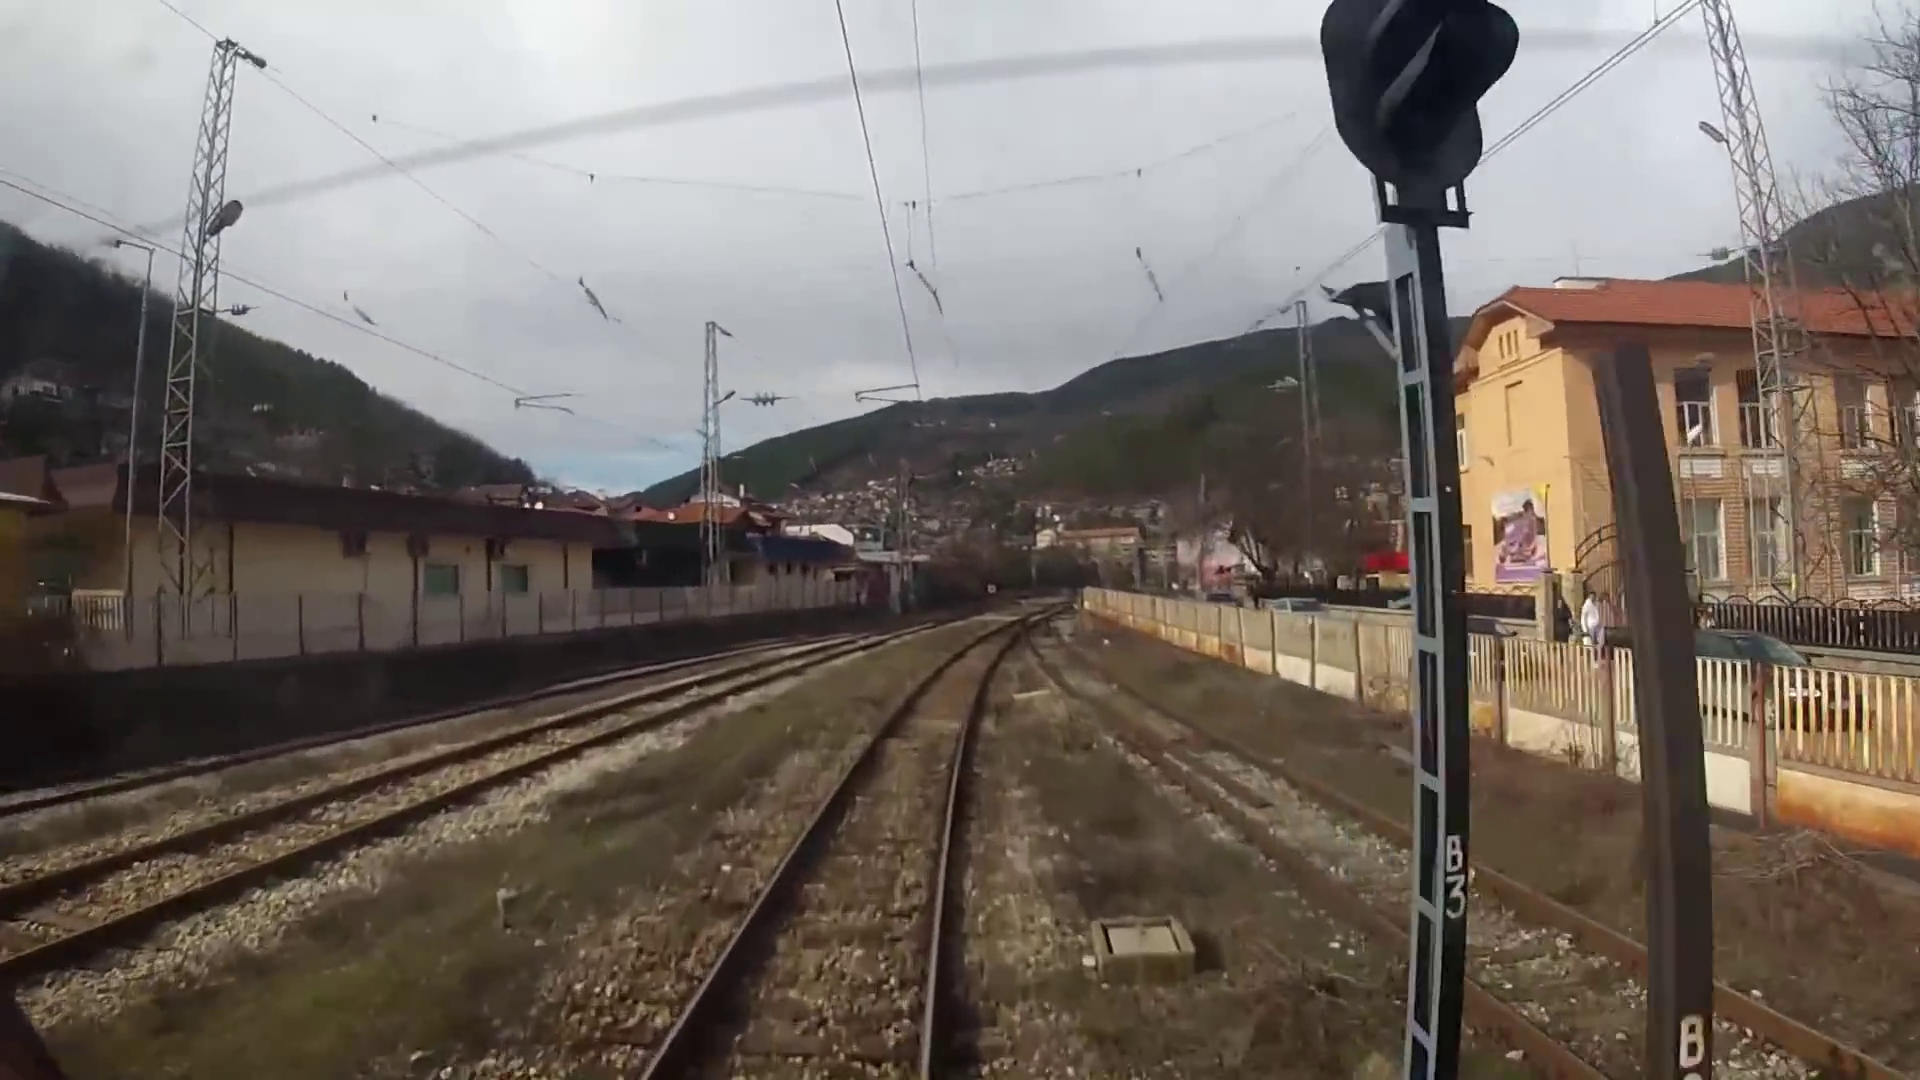
\includegraphics[width=30mm]{src/img/results-ml-0/par4/frame.jpg} & 
  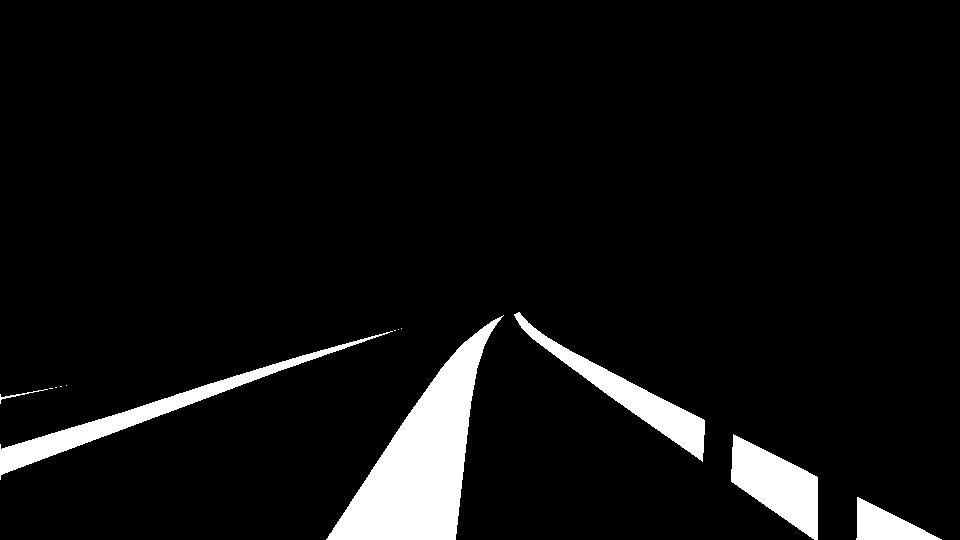
\includegraphics[width=30mm]{src/img/results-ml-0/par4/seg.jpeg} & 
  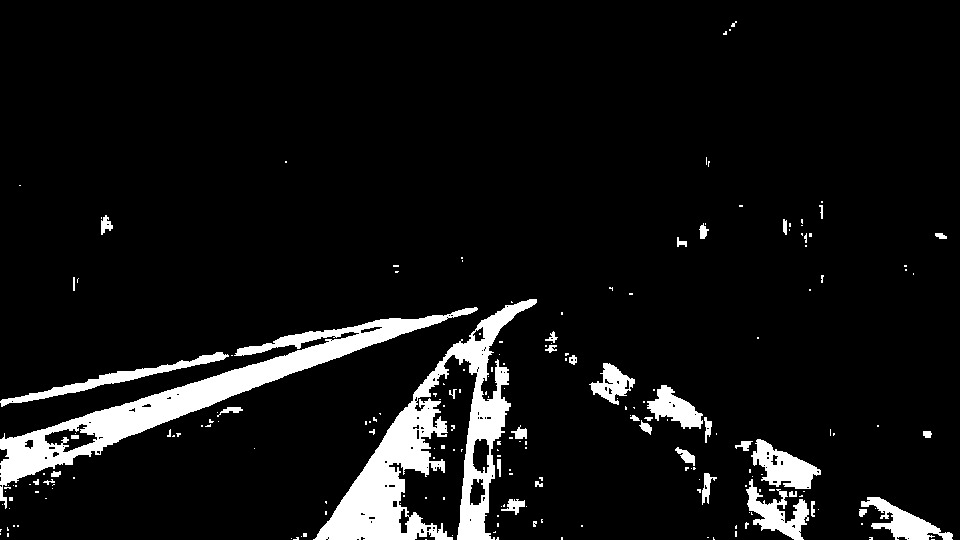
\includegraphics[width=30mm]{src/img/results-ml-0/par4/det.jpg} &
  rail-to-rail \\
  \multicolumn{4}{l}{(a) Training Dataset - RailSem19\cite{zendel2019railsem19} (Train Dash Cam) } \\ \hline
  
  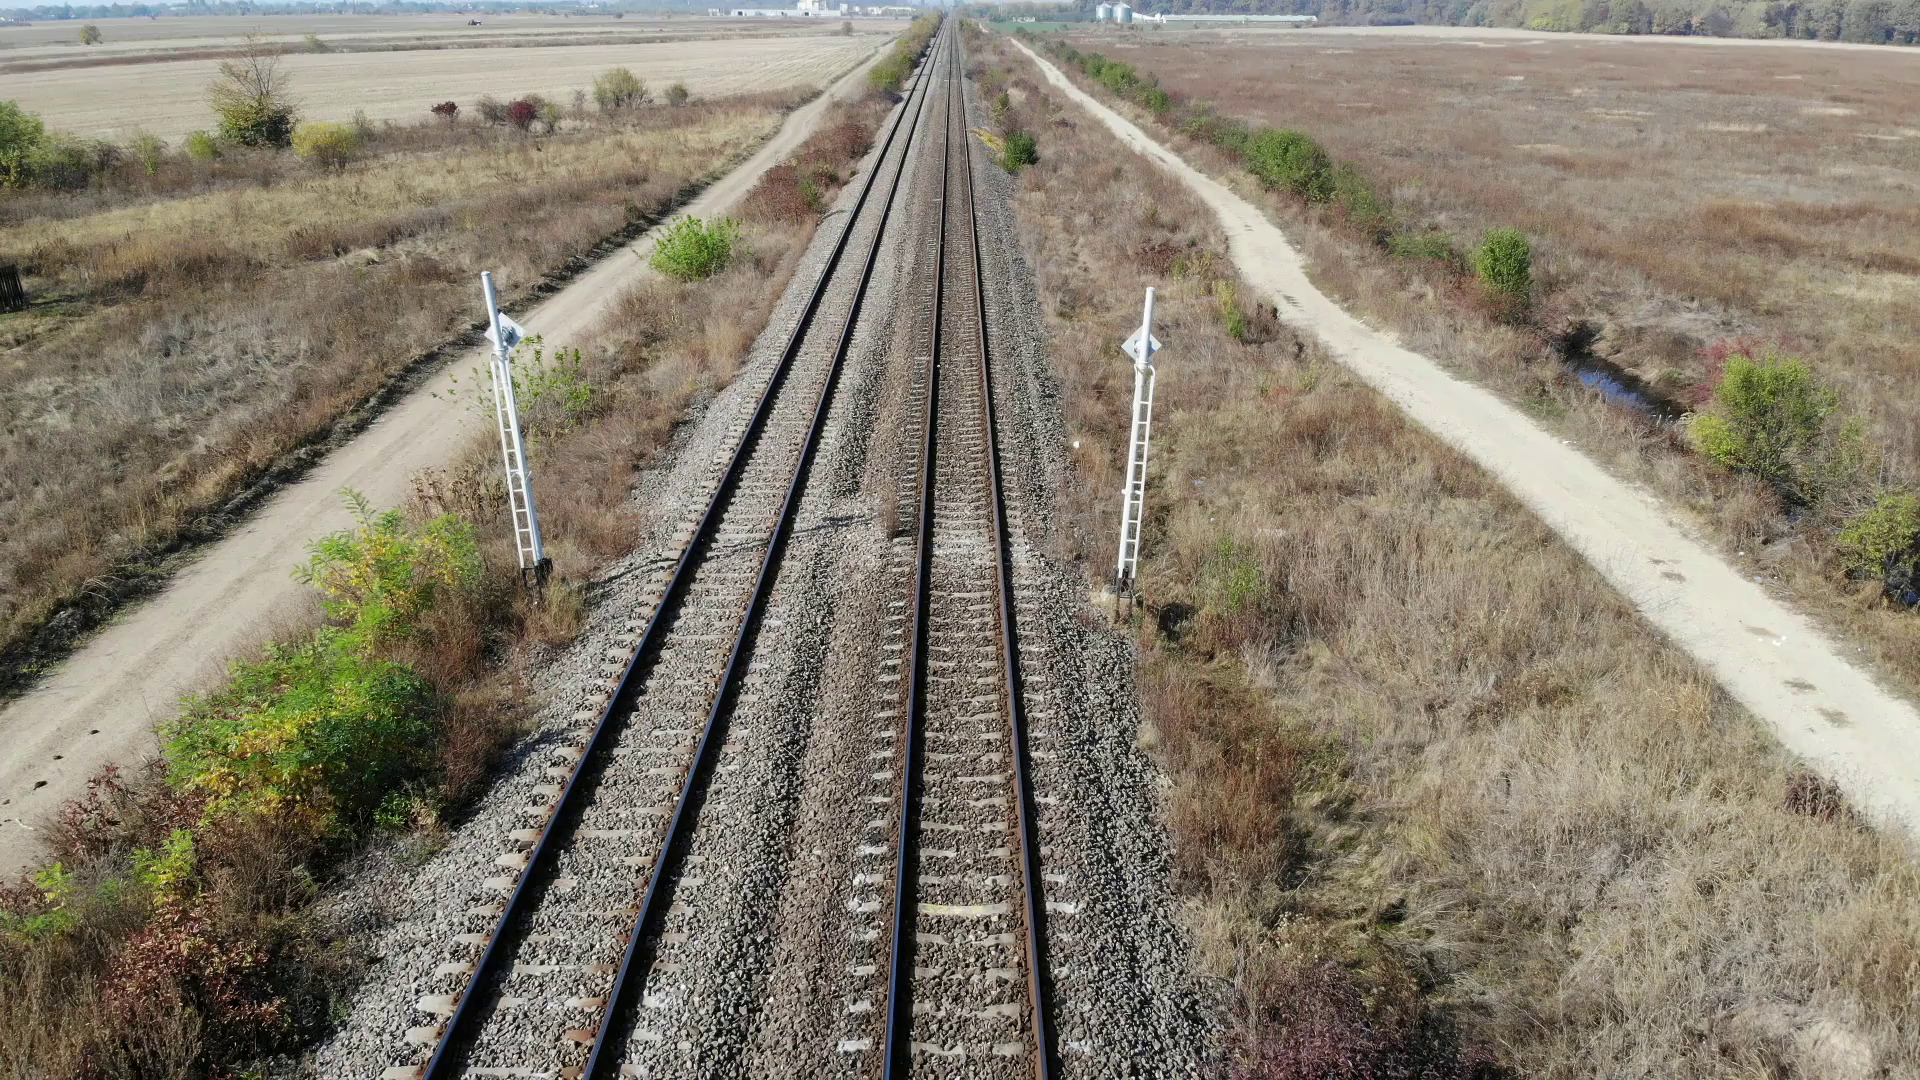
\includegraphics[width=30mm]{src/img/results-ml-0/par3/frame.jpg} & 
  
\includegraphics[width=30mm]{src/img/results-ml-0/par3/seg.jpg} & 
  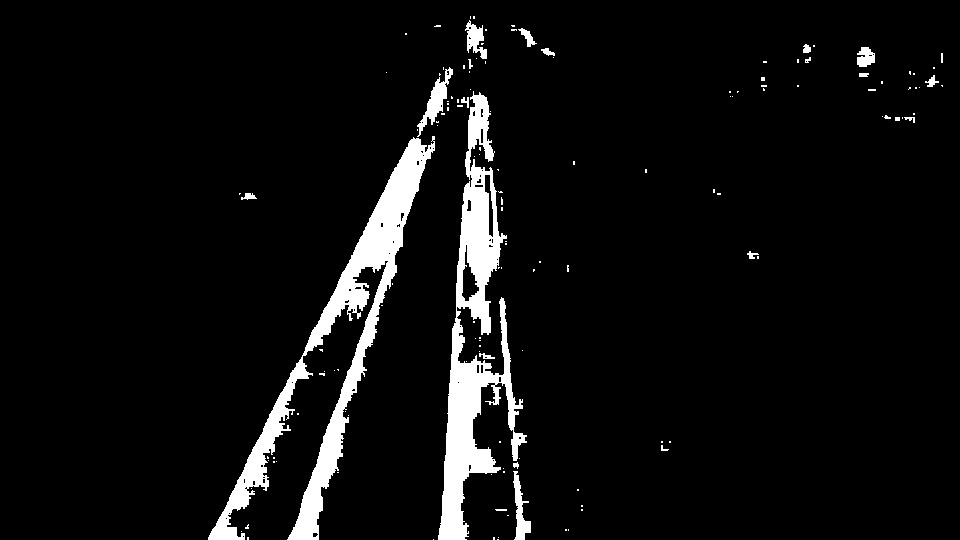
\includegraphics[width=30mm]{src/img/results-ml-0/par3/det.jpg} &
  rail-to-rail  \\
  \multicolumn{4}{l}{ (b) Validation Dataset \footnote{Obtained from an initiative of NETIO and Thales} (Drone Cam) } \\ \hline
  
  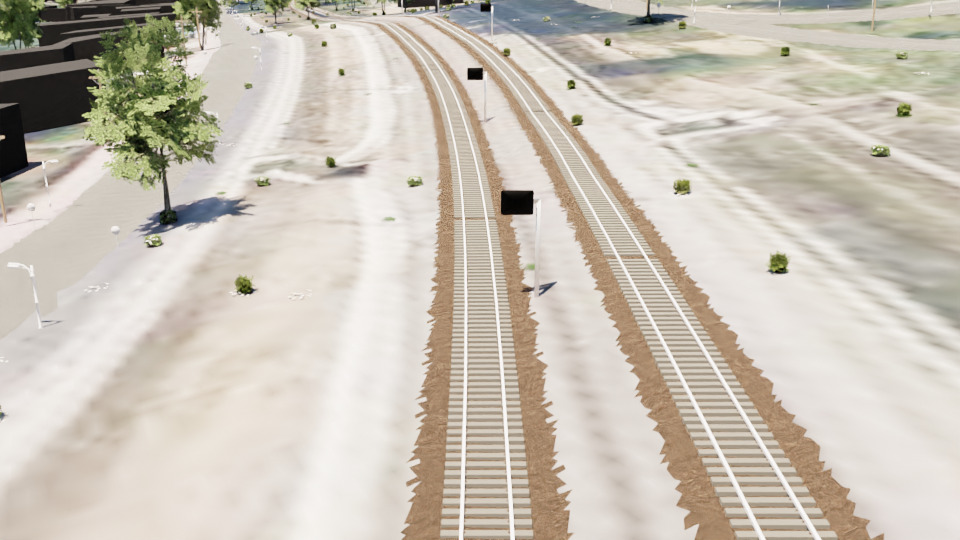
\includegraphics[width=30mm]{src/img/results-ml-0/par0/frame.jpg} & 
  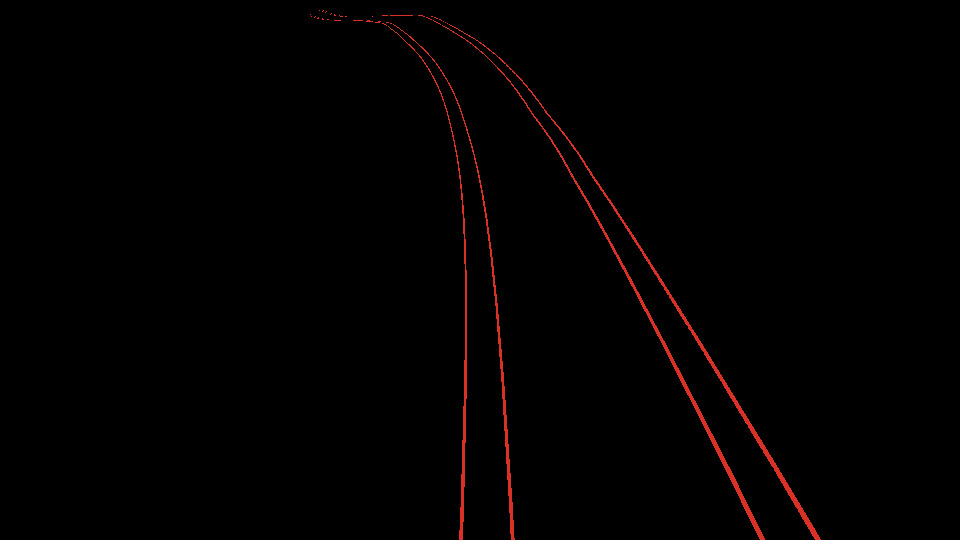
\includegraphics[width=30mm]{src/img/results-ml-0/par0/seg.jpg} & 
  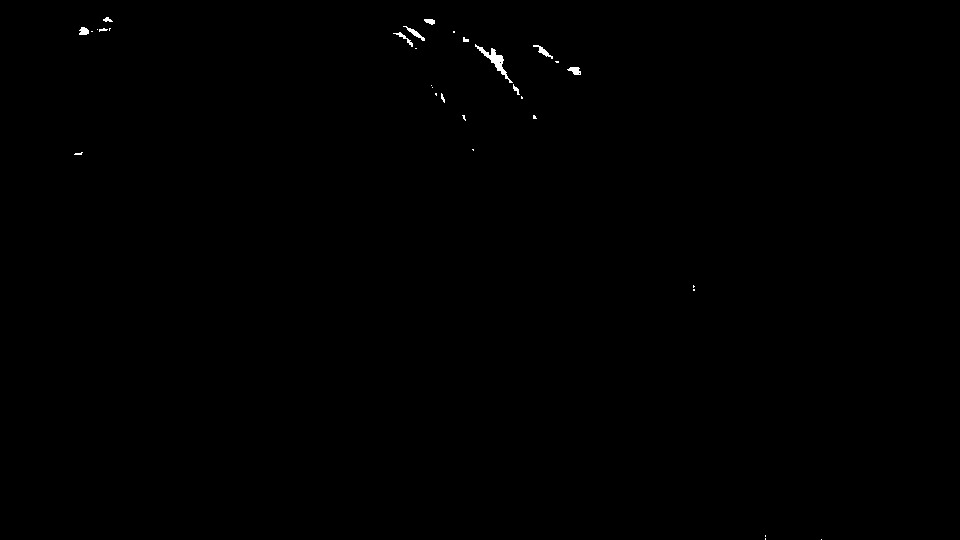
\includegraphics[width=30mm]{src/img/results-ml-0/par0/det.jpg} &
  rails only  \\
  \multicolumn{4}{l}{ (c) Initial Attempt } \\ \hline
  
  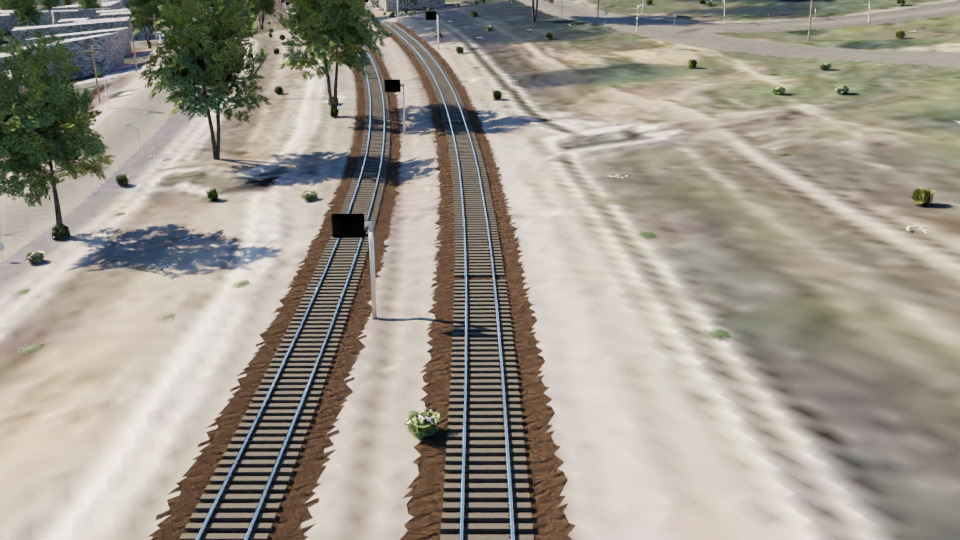
\includegraphics[width=30mm]{src/img/results-ml-0/par1/frame.jpg} & 
  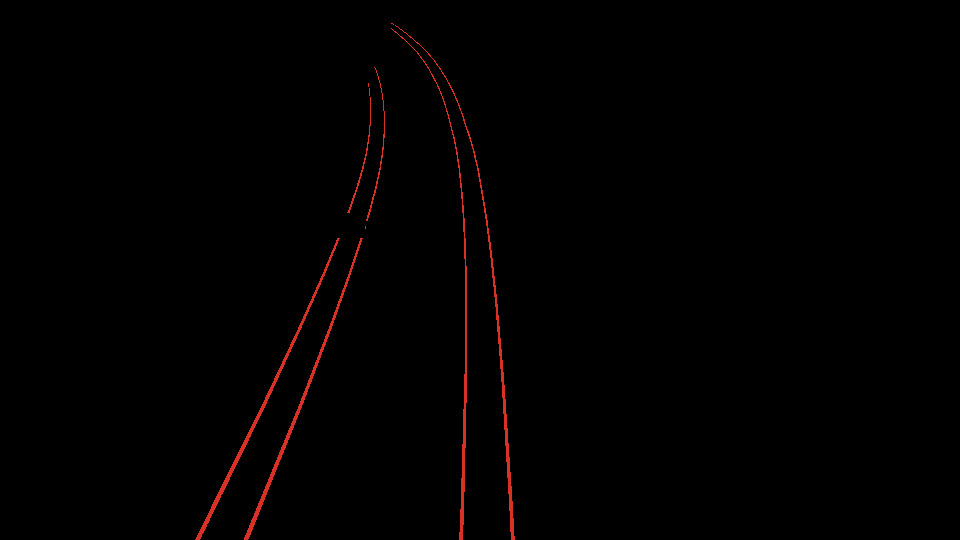
\includegraphics[width=30mm]{src/img/results-ml-0/par1/seg.jpg} & 
  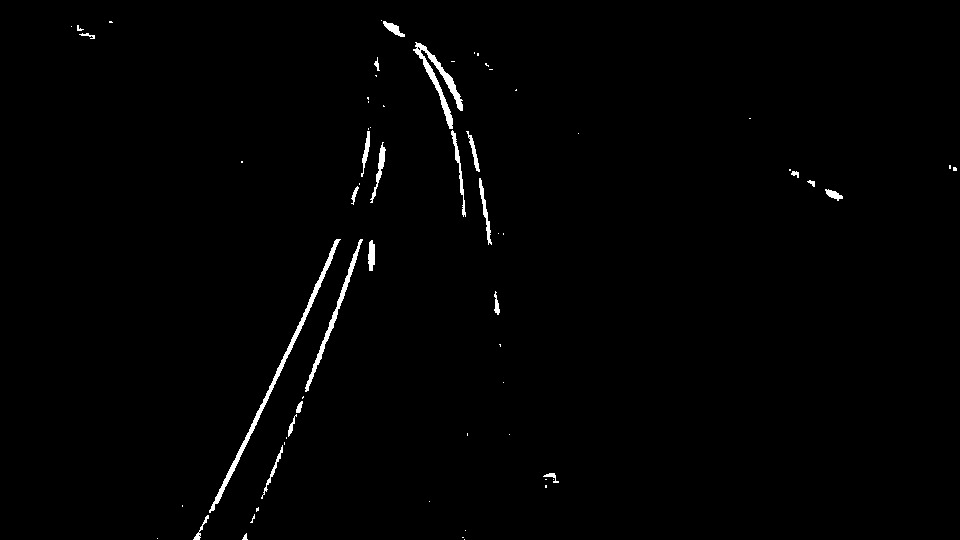
\includegraphics[width=30mm]{src/img/results-ml-0/par1/det.jpg} &
  rails only  \\
  \multicolumn{4}{l}{   (d) Improved Rail Track Materials } \\ \hline
  
  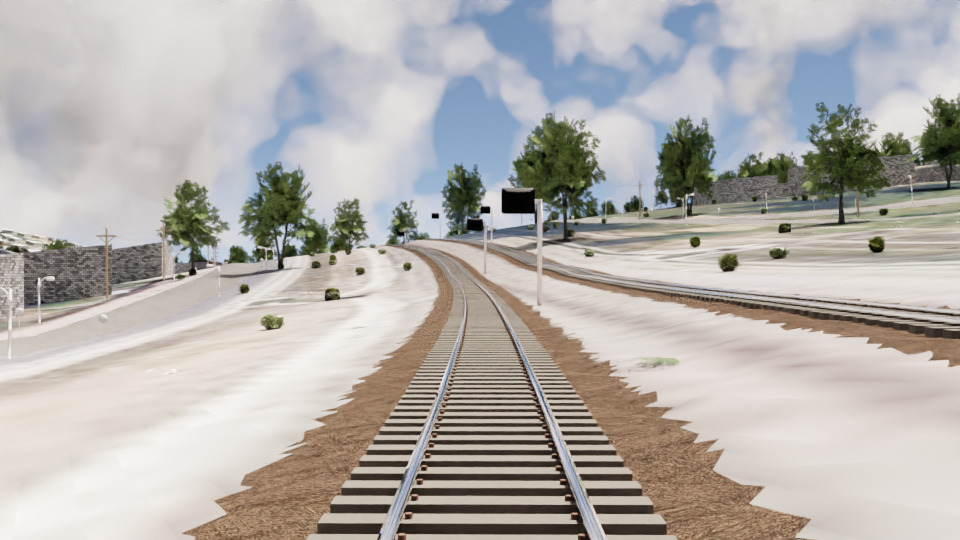
\includegraphics[width=30mm]{src/img/results-ml-0/par2/frame.jpg} & 
  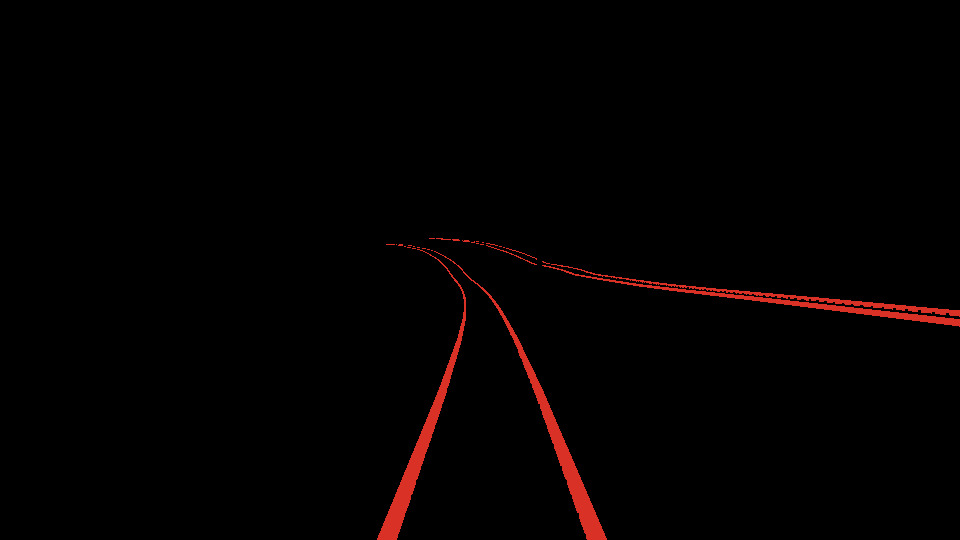
\includegraphics[width=30mm]{src/img/results-ml-0/par2/seg.jpg} & 
  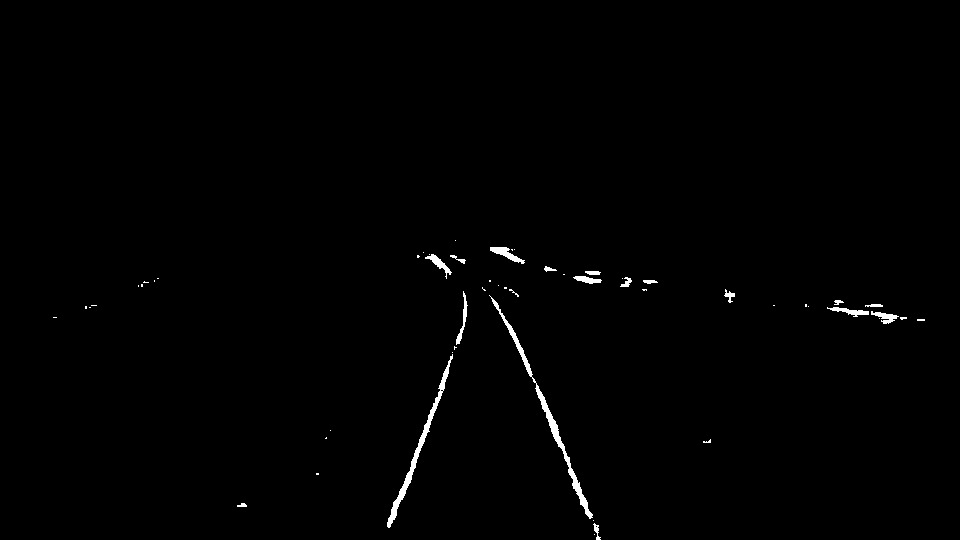
\includegraphics[width=30mm]{src/img/results-ml-0/par2/det.jpg} &
  rails only  \\
  \multicolumn{4}{l}{  (e) Adjusted Camera Angle, Added Clouds  } \\ \hline
  
  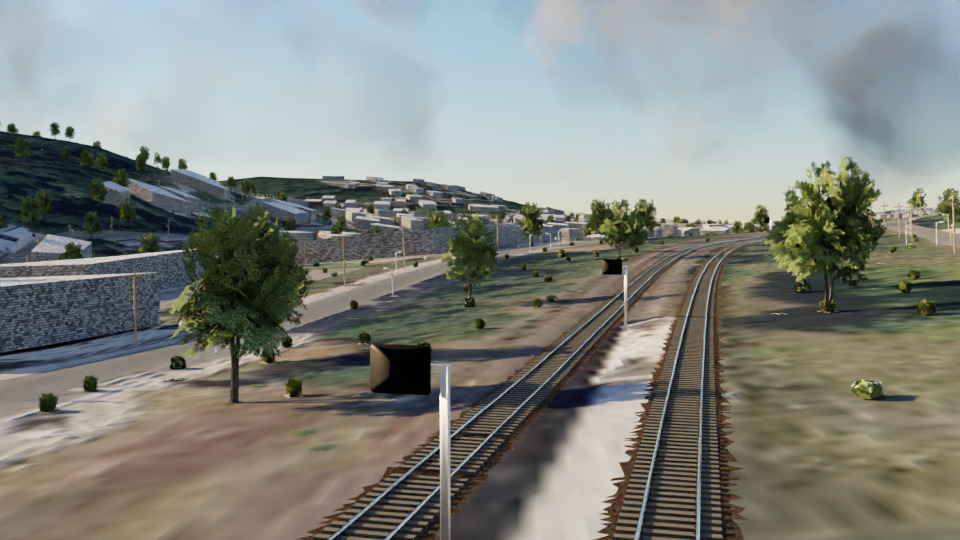
\includegraphics[width=30mm]{src/img/results-ml-0/par5/frame.jpg} & 
  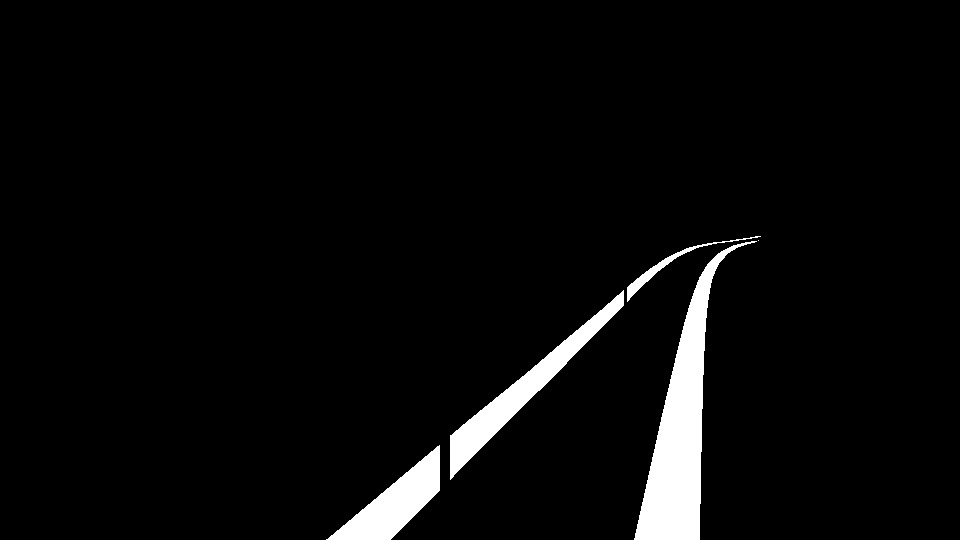
\includegraphics[width=30mm]{src/img/results-ml-0/par5/seg.jpg} & 
  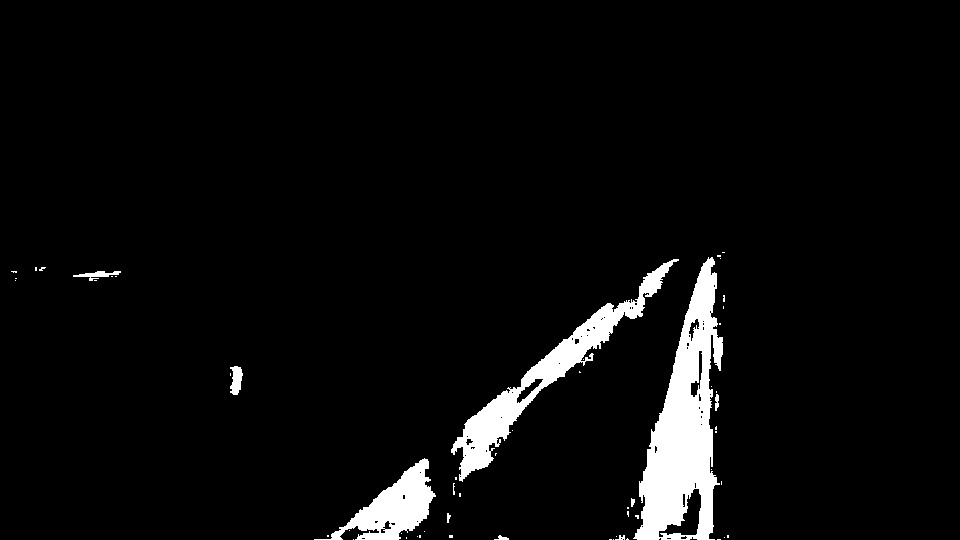
\includegraphics[width=30mm]{src/img/results-ml-0/par5/det.jpeg} &
  rail-to-rail  \\
  \multicolumn{4}{l}{  (f) Final Result  } \\
  
\end{tabular}
\caption{Evaluating the "unet" Machine Learning Model\cite{ALEXPETRE} on Real and Synthetic Frames}
\label{fig:ml-pics}
\end{table}

This synthetic data was used alongside real-world data from train dash cams\cite{zendel2019railsem19}, and drone footage \footnote{Obtained from an initiative of NETIO and Thales} of rail tracks. It is shown in \cite{ALEXPETRE} that the use of synthetic data alongside real data during training is beneficial to the performance of the model. These results are reproduced in Table \ref{fig:accuracy-improve}.

Two datasets have been created for this purpose. The first one, Dataset v1, makes use of all the features implemented for the scene generator, including volumetric clouds and vegetation scattering. At the request of the machine learning developers, we have removed volumetric clouds and all vegetation in a second version, Dataset v2. The second dataset also make use of Gamma normalization, to ensure the image exposure level is uniform across the entire dataset.

\begin{table}
\begin{tabular}{|l|c|}
\hline
  Data Used for Training & Model IoU Score \\ \hline
  Real data only & 87.39\%  \\
  Real data and Synthetic Dataset v1 (with trees and clouds) & 87.47\%  \\ 
  Real data and Synthetic Dataset v2 (no trees, normalized Gamma) & 87.49\%  \\
\hline
\end{tabular}
\caption{"unet" Model Accuracy Improvement from use with Synthetic Data\cite{ALEXPETRE}}
\label{fig:accuracy-improve}
\end{table}


\section{Evaluating Run Time and Data Size}
\label{sec:evaluate-runtime}


This section evaluates the runtime impact of each setting with respect to render time. A discussion of the Blender scene sizes and intermediate data sizes is also made. 


Since the rendering is done by a ray tracing algorithm, it is alike to a Monte Carlo Simulation: randomized rays of light are evaluated to obtain their impact on a specific pixel of the rendered image. In Blender, means the algorithm takes a variable time to finish, as early stopping is made when further iterations of the algorithm no longer affect the image in a meaningful way.

This means the render times are highly dependent on the scene: the number of objects visible, their complexity, but also local volumetric effects like clouds all affect the render time.

To evaluate scene build and render times in Table \ref{fig:run-time-table} we used 3D tiles of zoom levels 15, 17 and 18 to render train tracks in a resolution of 960x540. The rendering was done on a 6-core CPU model "Intel(R) Core(TM) i5-9400F @ 2.90GHz".

\begin{table}[H]
\centering
\begin{tabular}{|p{1.5cm}|p{1.5cm}|p{1.5cm}|p{3cm}|p{3cm}|}
\hline
    Render Trees? & Render Clouds? & Render Buildings? & Environment Generation Time (s) & Frame Render Time (s) \\
\hline
    False & False & False &  88.93 & 59.02 \\
\hline
    \textbf{True} & False & False & 180.51 & 61.44 \\
\hline
    False & \textbf{True} & False & 85.53 & 132.5 \\
\hline
    False & False & \textbf{True} & 110.28 & 55.34 \\
\hline
    \textbf{True} & False & \textbf{True} & 210.36 & 65.14 \\
\hline
    \textbf{True} & \textbf{True} & \textbf{True} & 193.82 & 123.13 \\
\hline
\end{tabular}
\caption{Scene Generation and Render Run Times}
\label{fig:run-time-table}
\end{table}

As shown in Table \ref{fig:run-time-table}, the cloud generation has the most impact on render time, and the vegetation generation has the most impact on scene generation time.

We have also used Blender's Nvidia CUDA renderer implementation with a GPU model "NVIDIA GeForce GTX 1660 Ti", and found a consistent 5-10\% improvement in render times, at the cost of a much slower environment generation time. This was caused by the shader compilation step, which for our use-case takes approximately 320 seconds.

Memory use, on the other hand, is more predictable. Our implementation of the rail track segmentation task uses 8-12 GB of RAM for rendering the scene, depending on the render parameters and scene settings.

\begin{table}[H]
\centering
\begin{tabular}{|p{4.5cm}|p{2.5cm}|p{7cm}|}
\hline
    Asset Type & Asset Size (MB) & Observations \\
\hline
    Downloaded 3D Tile & 30 - 100 & Larger or more densely urban tiles require more storage. \\
\hline
    Generated Environment Scene & 270 - 330 & Depends on tile size, count, and the 3D model library size. \\
\hline
    Rendered Frame Set & 1 - 4 & Depends on resolution. All outputs can be converted to JPEG to reduce storage requirements.  \\
\hline
\end{tabular}
\caption{Scene Generation and Render Run Times}
\label{fig:output-data-sizee}
\end{table}

Finally, we discuss the output data sizes for each stage of the project in table \ref{fig:output-data-sizee}. As mentioned in Section \ref{sec:dowonload-geo-data}, the raw GIS data is stored as 3D tiles. Then, a number of tiles centered on the same point are combined into an environment background scene. Finally, the environment scene is combined with more user assets and logic to render frames. 

